\documentclass{report}


\usepackage[T1]{fontenc}
\usepackage[utf8]{inputenc}
\usepackage{amsmath}


\usepackage{enumerate}

\usepackage{graphicx}
\usepackage{fancyhdr}
\usepackage{lettrine}
\usepackage{hyperref}
\usepackage{subcaption}
\usepackage{tikz}
\usepackage{cite}
\usepackage{listings}
\usepackage[nottoc, numbib]{tocbibind}
\usepackage[ngerman]{babel}
\usepackage[Glenn]{fncychap}
\usepackage{trfsigns}
\usepackage{parskip}
\usepackage{microtype}


\usetikzlibrary{shapes}
    \usetikzlibrary{arrows}
    \usetikzlibrary{arrows.meta,topaths}
    \usetikzlibrary{bending}
    \usetikzlibrary{calc}
\title{Elektrotechnik 1 Praktikum 1}


\usepackage[
  includehead,
  headheight = 17mm,
  footskip = \dimexpr\headsep+\ht\strutbox\relax,
  tmargin = 0mm,
  bmargin = \dimexpr17mm+2\ht\strutbox\relax,
]{geometry}

\usepackage{anyfontsize}
\usepackage{float}
\usepackage{xcolor}

\definecolor{DarkGreenBlue}{HTML}{264653}
\definecolor{LightGreenBlue}{HTML}{2A9D8F}
\definecolor{LightOrange}{HTML}{E9C46A}
\definecolor{DarkOrange}{HTML}{F4A261}
\definecolor{RedOrange}{HTML}{E76F51}
\definecolor{BrightRed}{HTML}{D62828}
\definecolor{DeepBlue}{HTML}{003049}

\lstdefinestyle{code}{
    backgroundcolor=\color{backcolour},
    commentstyle=\color{codegreen},
    keywordstyle=\color{magenta},
    numberstyle=\tiny\color{codegray},
    stringstyle=\color{codepurple},
    basicstyle=\ttfamily\footnotesize,
    breakatwhitespace=false,
    breaklines=true,
    captionpos=b,
    keepspaces=true,
    numbers=left,
    numbersep=5pt,
    showspaces=false,
    showstringspaces=false,
    showtabs=false,
    tabsize=2
}

\definecolor{codegreen}{rgb}{0,0.6,0}
\definecolor{codegray}{rgb}{0.5,0.5,0.5}
\definecolor{codepurple}{rgb}{0.502,0.502,0.0}
\definecolor{backcolour}{rgb}{0.95,0.95,0.95}

\lstdefinelanguage{ST}
{
	morekeywords={
	case,of,if,then,end_if,end_case,super,function_block,extends,var,
	constant, byte,,end_var,var_input, real,bool,var_output,
	dint,udint,word,dword,array, of,uint,not,adr, program, for, end_for, while, do, end_while, repeat, end_repeat, until, to, by, else, elsif
	},
	otherkeywords={
		:, :=, <>,;,\,.,\[,\],\^,1,2,3,4,5,6,7,8,9,0, TRUE, FALSE, \{attribute,  \'hide\'\}
	},
	keywords=[1]{
		case,of,if,then,end_if,end_case,super,function_block,extends,var,
		constant, byte,,end_var,var_input, real,bool,var_output,
		dint,udint,word,dword,array, of,uint,not,adr, :, :=, <>,;,\,.,\[,\],\^,program, for, end_for, while, do, end_while, repeat, end_repeat, until, to, by, else, elsif
	},
	keywordstyle=[1]\color{blue},
	keywords=[2]{
		1,2,3,4,5,6,7,8,9,0, TRUE, FALSE
	},
	keywordstyle=[2]\color{codepurple},
	keywords=[3]{
		\{attribute,  \'hide\'\}
	},
	keywordstyle=[3]\color{codegray},
	sensitive=false,
	morecomment=[l]{//},
	morecomment=[s]{(*}{*)},
	morestring=[b]"
	morestring=[b]'
}

\lstset{
	language={ST},
	backgroundcolor=\color{backcolour},
	commentstyle=\color{codegreen}\textit,
	keywordstyle=\color{blue},
	numberstyle=\tiny\color{codegray},
	stringstyle=\color{codepurple},
	basicstyle=\ttfamily\scriptsize,
	breakatwhitespace=false,
	breaklines=true,
	captionpos=b,
	keepspaces=true,
	numbers=left,
	numbersep=5pt,
	showspaces=false,
	showstringspaces=false,
	showtabs=false,
	tabsize=2
}
\pagestyle{fancy}
\fancyhead[L]{\leftmark}
\fancyhead[R]{}
\fancyfoot[L]{}
\fancyfoot[C]{\thepage}
%\fancyfoot[R]{\includegraphics[scale=0.2]{../assets/images/haw.jpg}}
\renewcommand\headrulewidth{0.5pt}


\begin{document}


\thispagestyle{empty}
\begin{tikzpicture}[overlay,remember picture]
  \thispagestyle{empty}
  \fill[black!2] (current page.south west) rectangle (current page.north east);

  \begin{scope}[transform canvas ={rotate around ={45:($(current page.north west)+(-.5,-6)$)}}]

    \shade[rounded corners=18pt, left color=DarkGreenBlue, right color=LightGreenBlue] ($(current page.north west)+(-.5,-6)$) rectangle ++(9,1.5);

  \end{scope}

  \begin{scope}[transform canvas ={rotate around ={45:($(current page.north west)+(.5,-10)$)}}]

    \shade[rounded corners=18pt, left color=LightOrange,right color=DarkOrange] ($(current page.north west)+(0.5,-10)$) rectangle ++(15,1.5);

  \end{scope}

  \begin{scope}[transform canvas ={rotate around ={45:($(current page.north west)+(0.5,-10)$)}}]

    \shade[rounded corners=8pt, right color=DarkOrange, left color=LightOrange] ($(current page.north west)+(1.5,-9.55)$) rectangle ++(7,.6);

  \end{scope}

  \begin{scope}[transform canvas ={rotate around ={45:($(current page.north)+(-1.5,-3)$)}}]

    \shade[rounded corners=12pt, left color=DeepBlue!80, right color=DeepBlue!60] ($(current page.north)+(-1.5,-3)$) rectangle ++(9,0.8);

  \end{scope}

  \begin{scope}[transform canvas ={rotate around ={45:($(current page.north)+(-3,-8)$)}}]

    \shade[rounded corners=28pt, left color=BrightRed, right color=BrightRed!80] ($(current page.north)+(-3,-8)$) rectangle ++(15,1.8);

  \end{scope}

  \begin{scope}[transform canvas ={rotate around ={45:($(current page.north west)+(4,-15.5)$)}}]

    \shade[rounded corners=25pt, left color=RedOrange, right color=DarkOrange] ($(current page.north west)+(4,-15.5)$) rectangle ++(30,1.8);

  \end{scope}

  \begin{scope}[transform canvas ={rotate around ={45:($(current page.north west)+(13,-10)$)}},]

    \shade[rounded corners=22pt, left color=DeepBlue,right color=DarkGreenBlue] ($(current page.north west)+(13,-10)$) rectangle ++(15,1.5);

  \end{scope}

  \begin{scope}[transform canvas ={rotate around ={45:($(current page.north west)+(18,-8)$)}},]

    \shade[rounded corners=8pt, left color=DarkOrange] ($(current page.north west)+(18,-8)$) rectangle ++(15,0.6);

  \end{scope}

  \begin{scope}[transform canvas ={rotate around ={45:($(current page.north west)+(19,-5.65)$)}},]

    \shade[rounded corners=12pt, left color=RedOrange] ($(current page.north west)+(19,-5.65)$) rectangle ++(15,0.8);

  \end{scope}

  \begin{scope}[transform canvas ={rotate around ={45:($(current page.north west)+(20,-9)$)}}]

    \shade[rounded corners=20pt, left color=BrightRed, right color=BrightRed!80] ($(current page.north west)+(20,-9)$) rectangle ++(14,1.2);

  \end{scope}

  \draw[ultra thick,gray] ($(current page.center)+(5,2)$) -- ++(0,-3cm) node[midway,left=0.25cm,text width=5cm,align=right,black!75]{{\fontsize{25}{30} \selectfont \bf PA\\[10pt] Doku}} node[midway,right=0.25cm,text width=6cm,align=left,orange]{{\fontsize{70}{86} \selectfont 2023}};

  \node at ($(current page.center)+(0,-4)$) {{\fontsize{40}{72} \selectfont PA: Transportarm}};

  \node[text width=8cm,align=center] at ($(current page.center)+(0,-6.5)$) {{\fontsize{16}{20} \selectfont \textcolor{orange}{ \bf \today}} \\[3pt] Emily Antosch 2519935};

\end{tikzpicture}

\newpage

\tableofcontents

\listoffigures

\newpage

\chapter{PA - Dokumentation des Transportarms}

\section{Dokumentation der Visualisierung}
\label{sec:einfuhrung}

\subsection{Beschreibung}

Das Programm ist in der Lage, die Funktion einer Lackiereinrichtung mit Transportarm zu simulieren. Die Visualisierung ist in Abbildung \ref{fig:visu} zu sehen. Die Anlage besteht aus zwei Bändern \textit{A} und \textit{E} und drei Stationen \textit{L1}, \textit{L2} und \textit{K}. Auf einem Transportband kommen die zu lackierenden Teile an. Die Station \textit{L1} ist die erste Lackierstation, an der die Teile lackiert werden. Die Station \textit{K} ist die Konservierstation, an der die Teile konserviert werden. Die Stationen \textit{L1}, \textit{L2} und \textit{K} sind jeweils mit einem Roboterarm ansteuerbar. Nachdem die Teile lackiert wurden, werden sie auf dem zweiten Transportband \textit{E} abgelegt. Die Station \textit{L2} ist die zweite Lackierstation, die die gleiche Funktion wie \textit{L1} übernimmt. 

Werkstücke können nur vorwärts durch die Anlage mit einem Transportarm bewegt werden. Es gibt, in der Version der Anlage, zwei Werkstücke, die in einem Durchlauf verarbeitet werden können. Ein Transport von einer Station zur nächsten dauert zwei Sekunden und jede Bearbeitung eines Werkstückes an einer Station dauert 5 Sekunden. Der Stand der Bearbeitung wird über eine Ampelanzeige erreicht. Die Ampel zeigt an, ob die Station frei ist, ob ein Werkstück bearbeitet wird oder ob ein Werkstück fertig bearbeitet worden ist. Dabei bedeutet Grün, dass die Station frei ist, Gelb, dass die Station die Arbeit abgeschlossen hat und Rot, dass die Bearbeitung des Werkstücks noch nicht beendet ist. Nur ein Werkstück kann gleichzeitig an einer Station liegen. Die Ampelanzeigen an den Bändern haben nur die Zustände Grün und Rot. Grün an der Station \textit{E} bedeutet, dass ein Werkstück zur Abholung bereit ist, während Rot bedeutet, dass das Band leer ist. Umgekehrt heißt Grün an der Station \textit{A}, dass die Station frei zur Abgabe eines Werkstücks ist und Rot, dass die Station noch nicht bereit für eine weitere Annahme ist (Band voll).

\begin{figure}
  \centering
  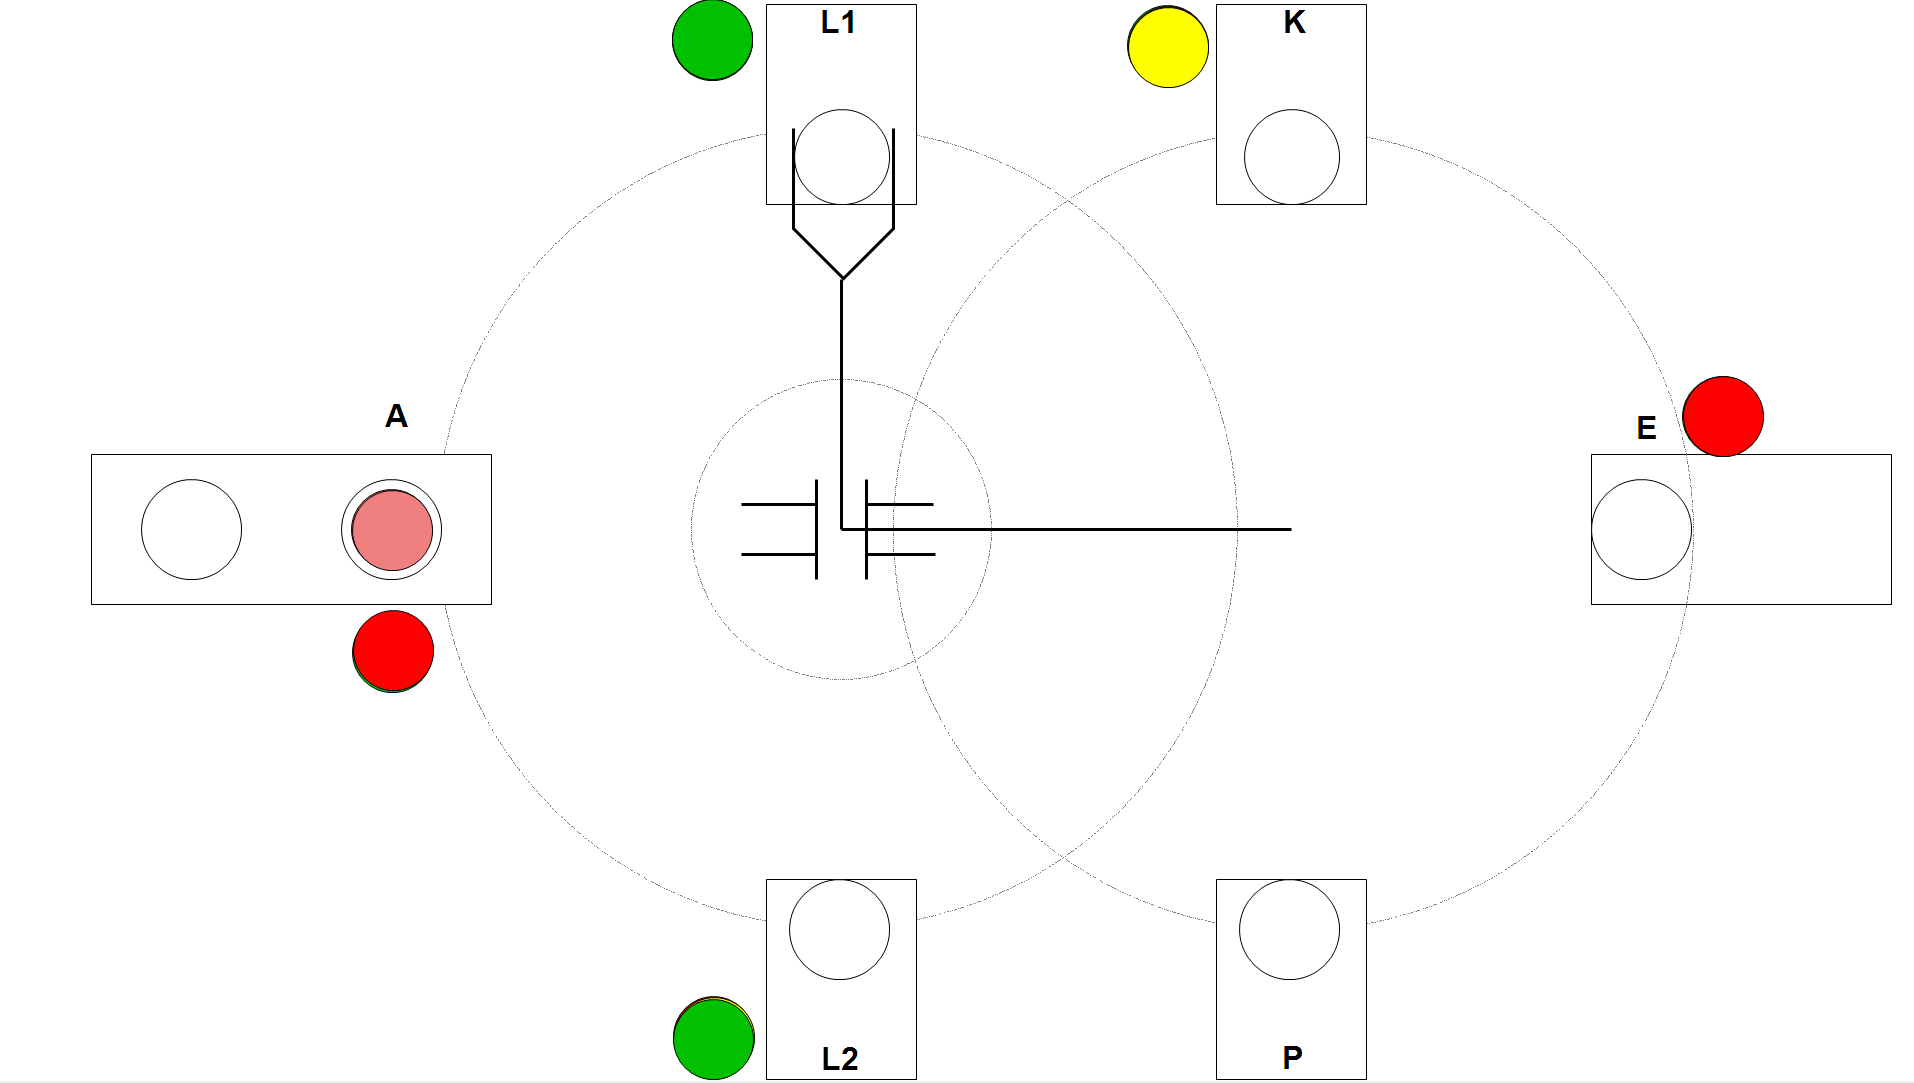
\includegraphics[width=0.8\textwidth]{assets/img/visu_v1.png}
  \caption{Visualisierung der Lackieranlage}
  \label{fig:visu}
\end{figure}

\subsection{Softwarekonzept}

Die Steuerung nimmt für die Visualisierung des Prozesses einen objektorientierten Ansatz. Der FB \textit{ArmModel} stellt dabei das Herz der Anwendung dar und managet die Bewegung des Arm innerhalb der Laufzeit des Programms. Der Status der Anlage wird über die ENUM \textit{ArmModelState} geregelt. In \textit{ArmModel} werden beim Start zunächst alle Werte zurückgesetzt und dann wird direkt in den Zustand \textit{NormalOperation} gewechselt. Dort wird fortlaufend überprüft, ob eine der Trigger gesetzt wurden, die das Bewegen von einem Werkstück von A nach B einleiten. Ist dies der Fall, werden zunächst verschiedene Informationen über den Transport gesammelt, um die richtige Bewegung ausführen zu können. Dazu gehören die Ausgangsposition des Werkstücks und das Ziel. Dann wird eine Animation ausgeführt, die in dem FB \textit{ProductionObject} definiert ist, ausgeführt. Jede weiterer Transport wird gesperrt, sodass sich immer nur ein Werkstück im Transport befinden kann. Am Ende des Transports werden die jeweiligen Zustände des Werkstücks, wie zum Beispiel die derzeitige Position, aktualisiert und die entsprechenden Stationen (\textit{ProductionStation}) werden darüber informiert, dass sie entweder ein Werkstück verloren haben oder ein neues dazugewonnen haben. Gleichzeitig führt die neue Station des Werkstücks ihre jeweilige Funktion aus. Ein Öffnen der Klammern um ein Objekt ist nicht notwendig um einen Transport zu veranlassen. Das könnte jedoch durch eine Erweiterung hinzugefügt werden. Zurzeit muss ein solcher Bewegungsbefehl über die Force-Tabelle erfolgen. Eine Steuerung könnte also nun über die Visualisierung gelegt werden, die diesen Prozess steuert und auch automatisiert.

Die Variablen, die gesetzt werden können, um einen Transport von einer Station zur nächsten zu veranlassen, sind:

\begin{itemize}
  \item \textit{ArmModel.MoveToL1}
  \item \textit{ArmModel.MoveToL2}
  \item \textit{ArmModel.MoveToKfromL1}
  \item \textit{ArmModel.MoveToKfromL2}
  \item \textit{ArmModel.MoveToE}
\end{itemize}

Bestimmte Konzepte zum Ablauf des Prozess sind bereits implementiert. So wird ein Bewegungsbefehl nicht ausgeführt, wenn dieser zu einer Kollision von zwei Werkstücken führen würde.

\subsection{Weitere Hinweise}

Sollte es ein Problem mit dem Programm und Unklarheiten bei der Bedienung geben, erreichen Sie mich unter: emilylucia.antosch@haw-hamburg.de. 

\end{document}
